\chapter{p4 = 8 (42 graphs)}
\newpage\begin{figure}
  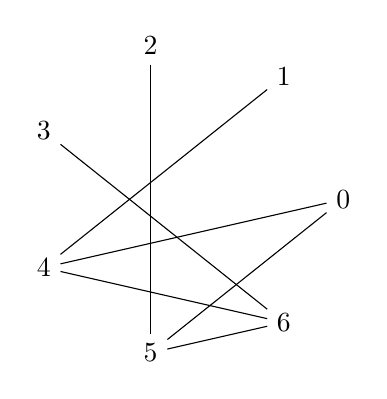
\begin{tikzpicture}
      \draw
        (0.0:2) node (0){0}
        (51.429:2) node (1){1}
        (102.857:2) node (2){2}
        (154.286:2) node (3){3}
        (205.714:2) node (4){4}
        (257.143:2) node (5){5}
        (308.571:2) node (6){6};
      \begin{scope}[-]
        \draw (0) to (4);
        \draw (0) to (5);
        \draw (1) to (4);
        \draw (2) to (5);
        \draw (3) to (6);
        \draw (4) to (6);
        \draw (5) to (6);
      \end{scope}
    \end{tikzpicture}
\end{figure}
\begin{itemize}
\item signature: 000110001000010001011
\item g: Graph with 7 nodes and 7 edges
\item order: 7
\item size: 7
\item max degree: 3
\item degrees: 1,1,1,2,3,3,3
\item is tree: 0
\item is bipartite: 1
\item has bridge: 1
\item is chordal: 0
\item is complete: 0
\item min cycle basis weight: 4
\item min cycle basis size: 1
\item diameter: 4
\item radius: 2
\item is eulerian: 0
\item is planar: 1
\item number of faces: 2
\item is regular: 0
\item p3: 10
\item p4: 8
\item property hash: a84dc7f826c26afc77595e6121fa6675bee536571a90d6a5aedbd831a3ca2128
\end{itemize}
\newpage
\begin{figure}
  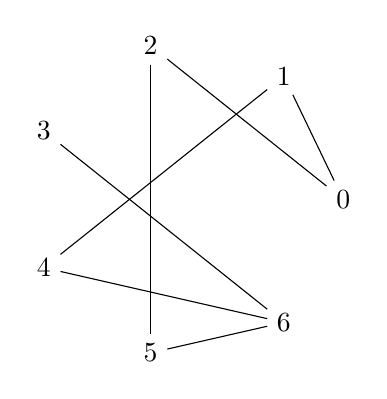
\begin{tikzpicture}
      \draw
        (0.0:2) node (0){0}
        (51.429:2) node (1){1}
        (102.857:2) node (2){2}
        (154.286:2) node (3){3}
        (205.714:2) node (4){4}
        (257.143:2) node (5){5}
        (308.571:2) node (6){6};
      \begin{scope}[-]
        \draw (0) to (1);
        \draw (0) to (2);
        \draw (1) to (4);
        \draw (2) to (5);
        \draw (3) to (6);
        \draw (4) to (6);
        \draw (5) to (6);
      \end{scope}
    \end{tikzpicture}
\end{figure}
\begin{itemize}
\item signature: 110000001000010001011
\item g: Graph with 7 nodes and 7 edges
\item order: 7
\item size: 7
\item max degree: 3
\item degrees: 1,2,2,2,2,2,3
\item is tree: 0
\item is bipartite: 1
\item has bridge: 1
\item is chordal: 0
\item is complete: 0
\item min cycle basis weight: 6
\item min cycle basis size: 1
\item diameter: 4
\item radius: 3
\item is eulerian: 0
\item is planar: 1
\item number of faces: 2
\item is regular: 0
\item p3: 8
\item p4: 8
\item property hash: 055727ab3388792762a5c4023cf5109aa052d17c81640271ee37c797d4715393
\end{itemize}
\newpage
\begin{figure}
  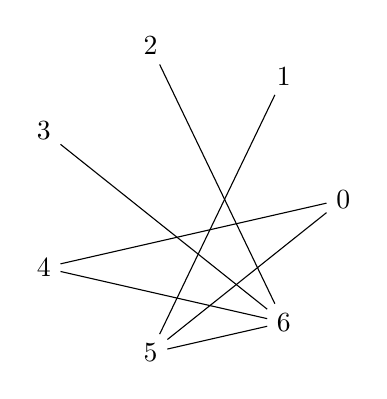
\begin{tikzpicture}
      \draw
        (0.0:2) node (0){0}
        (51.429:2) node (1){1}
        (102.857:2) node (2){2}
        (154.286:2) node (3){3}
        (205.714:2) node (4){4}
        (257.143:2) node (5){5}
        (308.571:2) node (6){6};
      \begin{scope}[-]
        \draw (0) to (4);
        \draw (0) to (5);
        \draw (1) to (5);
        \draw (2) to (6);
        \draw (3) to (6);
        \draw (4) to (6);
        \draw (5) to (6);
      \end{scope}
    \end{tikzpicture}
\end{figure}
\begin{itemize}
\item signature: 000110000100001001011
\item g: Graph with 7 nodes and 7 edges
\item order: 7
\item size: 7
\item max degree: 4
\item degrees: 1,1,1,2,2,3,4
\item is tree: 0
\item is bipartite: 1
\item has bridge: 1
\item is chordal: 0
\item is complete: 0
\item min cycle basis weight: 4
\item min cycle basis size: 1
\item diameter: 3
\item radius: 2
\item is eulerian: 0
\item is planar: 1
\item number of faces: 2
\item is regular: 0
\item p3: 11
\item p4: 8
\item property hash: d9113a7b2b2ce616bc7ca79f3ffb15f10153db48dbaf26229f960387e539802d
\end{itemize}
\newpage
\begin{figure}
  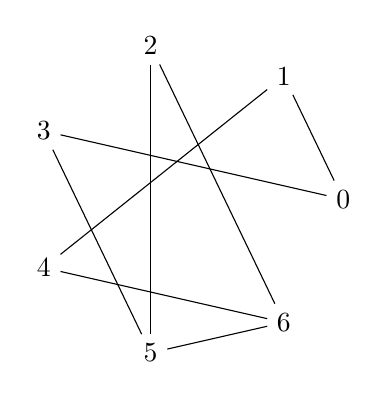
\begin{tikzpicture}
      \draw
        (0.0:2) node (0){0}
        (51.429:2) node (1){1}
        (102.857:2) node (2){2}
        (154.286:2) node (3){3}
        (205.714:2) node (4){4}
        (257.143:2) node (5){5}
        (308.571:2) node (6){6};
      \begin{scope}[-]
        \draw (0) to (1);
        \draw (0) to (3);
        \draw (1) to (4);
        \draw (2) to (5);
        \draw (2) to (6);
        \draw (3) to (5);
        \draw (4) to (6);
        \draw (5) to (6);
      \end{scope}
    \end{tikzpicture}
\end{figure}
\begin{itemize}
\item signature: 101000001000011010011
\item g: Graph with 7 nodes and 8 edges
\item order: 7
\item size: 8
\item max degree: 3
\item degrees: 2,2,2,2,2,3,3
\item is tree: 0
\item is bipartite: 0
\item has bridge: 0
\item is chordal: 0
\item is complete: 0
\item min cycle basis weight: 9
\item min cycle basis size: 2
\item diameter: 3
\item radius: 3
\item is eulerian: 0
\item is planar: 1
\item number of faces: 3
\item is regular: 0
\item p3: 8
\item p4: 8
\item property hash: de16d62120ac490765f4a295ff69794016f9938f4448c0aab7a91f88ab001ab7
\end{itemize}
\newpage
\begin{figure}
  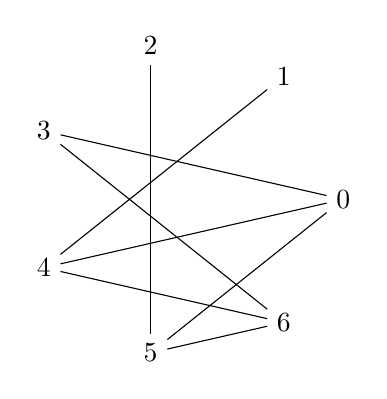
\begin{tikzpicture}
      \draw
        (0.0:2) node (0){0}
        (51.429:2) node (1){1}
        (102.857:2) node (2){2}
        (154.286:2) node (3){3}
        (205.714:2) node (4){4}
        (257.143:2) node (5){5}
        (308.571:2) node (6){6};
      \begin{scope}[-]
        \draw (0) to (3);
        \draw (0) to (4);
        \draw (0) to (5);
        \draw (1) to (4);
        \draw (2) to (5);
        \draw (3) to (6);
        \draw (4) to (6);
        \draw (5) to (6);
      \end{scope}
    \end{tikzpicture}
\end{figure}
\begin{itemize}
\item signature: 001110001000010001011
\item g: Graph with 7 nodes and 8 edges
\item order: 7
\item size: 8
\item max degree: 3
\item degrees: 1,1,2,3,3,3,3
\item is tree: 0
\item is bipartite: 1
\item has bridge: 1
\item is chordal: 0
\item is complete: 0
\item min cycle basis weight: 8
\item min cycle basis size: 2
\item diameter: 4
\item radius: 2
\item is eulerian: 0
\item is planar: 1
\item number of faces: 3
\item is regular: 0
\item p3: 13
\item p4: 8
\item property hash: 16c3951aa7af33fa11206867b868bb8670c46022d07f6e609f6d55e9c099b713
\end{itemize}
\newpage
\begin{figure}
  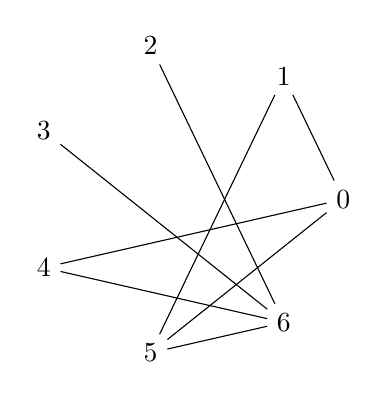
\begin{tikzpicture}
      \draw
        (0.0:2) node (0){0}
        (51.429:2) node (1){1}
        (102.857:2) node (2){2}
        (154.286:2) node (3){3}
        (205.714:2) node (4){4}
        (257.143:2) node (5){5}
        (308.571:2) node (6){6};
      \begin{scope}[-]
        \draw (0) to (1);
        \draw (0) to (4);
        \draw (0) to (5);
        \draw (1) to (5);
        \draw (2) to (6);
        \draw (3) to (6);
        \draw (4) to (6);
        \draw (5) to (6);
      \end{scope}
    \end{tikzpicture}
\end{figure}
\begin{itemize}
\item signature: 100110000100001001011
\item g: Graph with 7 nodes and 8 edges
\item order: 7
\item size: 8
\item max degree: 4
\item degrees: 1,1,2,2,3,3,4
\item is tree: 0
\item is bipartite: 0
\item has bridge: 1
\item is chordal: 0
\item is complete: 0
\item min cycle basis weight: 7
\item min cycle basis size: 2
\item diameter: 3
\item radius: 2
\item is eulerian: 0
\item is planar: 1
\item number of faces: 3
\item is regular: 0
\item p3: 11
\item p4: 8
\item property hash: 76cee932380a064e8e30a87663c9a4ae455e05884baa7fd15ef9651ed29eed8f
\end{itemize}
\newpage
\begin{figure}
  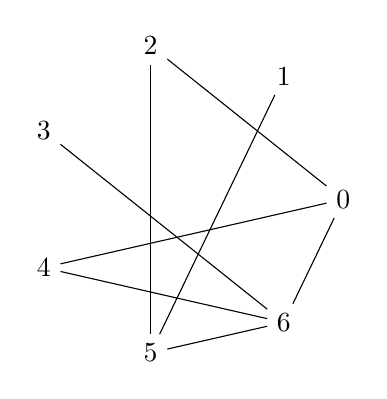
\begin{tikzpicture}
      \draw
        (0.0:2) node (0){0}
        (51.429:2) node (1){1}
        (102.857:2) node (2){2}
        (154.286:2) node (3){3}
        (205.714:2) node (4){4}
        (257.143:2) node (5){5}
        (308.571:2) node (6){6};
      \begin{scope}[-]
        \draw (0) to (2);
        \draw (0) to (4);
        \draw (0) to (6);
        \draw (1) to (5);
        \draw (2) to (5);
        \draw (3) to (6);
        \draw (4) to (6);
        \draw (5) to (6);
      \end{scope}
    \end{tikzpicture}
\end{figure}
\begin{itemize}
\item signature: 010101000100010001011
\item g: Graph with 7 nodes and 8 edges
\item order: 7
\item size: 8
\item max degree: 4
\item degrees: 1,1,2,2,3,3,4
\item is tree: 0
\item is bipartite: 0
\item has bridge: 1
\item is chordal: 0
\item is complete: 0
\item min cycle basis weight: 7
\item min cycle basis size: 2
\item diameter: 3
\item radius: 2
\item is eulerian: 0
\item is planar: 1
\item number of faces: 3
\item is regular: 0
\item p3: 11
\item p4: 8
\item property hash: 76cee932380a064e8e30a87663c9a4ae455e05884baa7fd15ef9651ed29eed8f
\end{itemize}
\newpage
\begin{figure}
  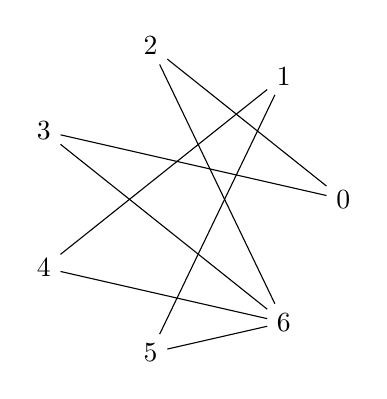
\begin{tikzpicture}
      \draw
        (0.0:2) node (0){0}
        (51.429:2) node (1){1}
        (102.857:2) node (2){2}
        (154.286:2) node (3){3}
        (205.714:2) node (4){4}
        (257.143:2) node (5){5}
        (308.571:2) node (6){6};
      \begin{scope}[-]
        \draw (0) to (2);
        \draw (0) to (3);
        \draw (1) to (4);
        \draw (1) to (5);
        \draw (2) to (6);
        \draw (3) to (6);
        \draw (4) to (6);
        \draw (5) to (6);
      \end{scope}
    \end{tikzpicture}
\end{figure}
\begin{itemize}
\item signature: 011000001100001001011
\item g: Graph with 7 nodes and 8 edges
\item order: 7
\item size: 8
\item max degree: 4
\item degrees: 2,2,2,2,2,2,4
\item is tree: 0
\item is bipartite: 1
\item has bridge: 0
\item is chordal: 0
\item is complete: 0
\item min cycle basis weight: 8
\item min cycle basis size: 2
\item diameter: 4
\item radius: 2
\item is eulerian: 1
\item is planar: 1
\item number of faces: 3
\item is regular: 0
\item p3: 12
\item p4: 8
\item property hash: 3a2c615f09b36ca255ed0d794ccc41ee159551325d4a9569b44d1e8ffa12afeb
\end{itemize}
\newpage
\begin{figure}
  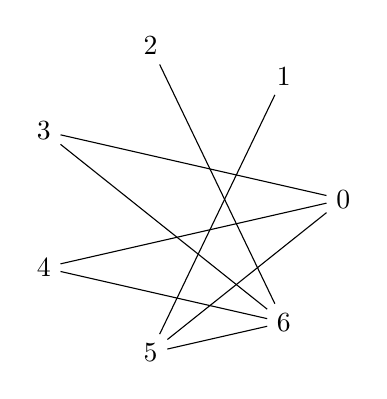
\begin{tikzpicture}
      \draw
        (0.0:2) node (0){0}
        (51.429:2) node (1){1}
        (102.857:2) node (2){2}
        (154.286:2) node (3){3}
        (205.714:2) node (4){4}
        (257.143:2) node (5){5}
        (308.571:2) node (6){6};
      \begin{scope}[-]
        \draw (0) to (3);
        \draw (0) to (4);
        \draw (0) to (5);
        \draw (1) to (5);
        \draw (2) to (6);
        \draw (3) to (6);
        \draw (4) to (6);
        \draw (5) to (6);
      \end{scope}
    \end{tikzpicture}
\end{figure}
\begin{itemize}
\item signature: 001110000100001001011
\item g: Graph with 7 nodes and 8 edges
\item order: 7
\item size: 8
\item max degree: 4
\item degrees: 1,1,2,2,3,3,4
\item is tree: 0
\item is bipartite: 1
\item has bridge: 1
\item is chordal: 0
\item is complete: 0
\item min cycle basis weight: 8
\item min cycle basis size: 2
\item diameter: 3
\item radius: 2
\item is eulerian: 0
\item is planar: 1
\item number of faces: 3
\item is regular: 0
\item p3: 14
\item p4: 8
\item property hash: 9acff7d3264adbe93b86f47ef41c8f47abace9da3cb90eebc05b8aee9e6ea0ab
\end{itemize}
\newpage
\begin{figure}
  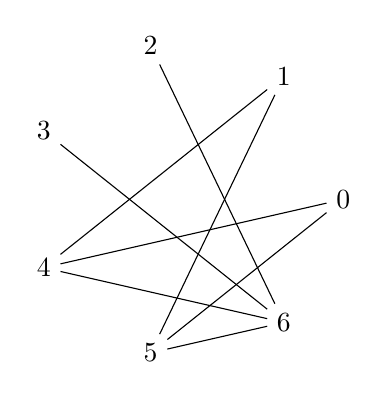
\begin{tikzpicture}
      \draw
        (0.0:2) node (0){0}
        (51.429:2) node (1){1}
        (102.857:2) node (2){2}
        (154.286:2) node (3){3}
        (205.714:2) node (4){4}
        (257.143:2) node (5){5}
        (308.571:2) node (6){6};
      \begin{scope}[-]
        \draw (0) to (4);
        \draw (0) to (5);
        \draw (1) to (4);
        \draw (1) to (5);
        \draw (2) to (6);
        \draw (3) to (6);
        \draw (4) to (6);
        \draw (5) to (6);
      \end{scope}
    \end{tikzpicture}
\end{figure}
\begin{itemize}
\item signature: 000110001100001001011
\item g: Graph with 7 nodes and 8 edges
\item order: 7
\item size: 8
\item max degree: 4
\item degrees: 1,1,2,2,3,3,4
\item is tree: 0
\item is bipartite: 1
\item has bridge: 1
\item is chordal: 0
\item is complete: 0
\item min cycle basis weight: 8
\item min cycle basis size: 2
\item diameter: 3
\item radius: 2
\item is eulerian: 0
\item is planar: 1
\item number of faces: 3
\item is regular: 0
\item p3: 14
\item p4: 8
\item property hash: 9acff7d3264adbe93b86f47ef41c8f47abace9da3cb90eebc05b8aee9e6ea0ab
\end{itemize}
\newpage
\begin{figure}
  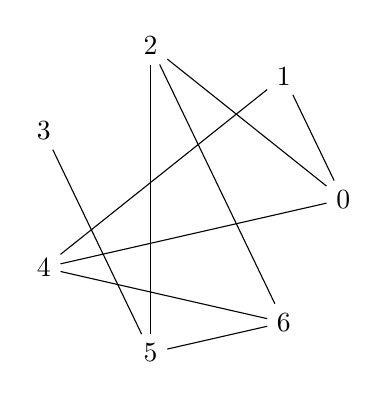
\begin{tikzpicture}
      \draw
        (0.0:2) node (0){0}
        (51.429:2) node (1){1}
        (102.857:2) node (2){2}
        (154.286:2) node (3){3}
        (205.714:2) node (4){4}
        (257.143:2) node (5){5}
        (308.571:2) node (6){6};
      \begin{scope}[-]
        \draw (0) to (1);
        \draw (0) to (2);
        \draw (0) to (4);
        \draw (1) to (4);
        \draw (2) to (5);
        \draw (2) to (6);
        \draw (3) to (5);
        \draw (4) to (6);
        \draw (5) to (6);
      \end{scope}
    \end{tikzpicture}
\end{figure}
\begin{itemize}
\item signature: 110100001000011010011
\item g: Graph with 7 nodes and 9 edges
\item order: 7
\item size: 9
\item max degree: 3
\item degrees: 1,2,3,3,3,3,3
\item is tree: 0
\item is bipartite: 0
\item has bridge: 1
\item is chordal: 0
\item is complete: 0
\item min cycle basis weight: 10
\item min cycle basis size: 3
\item diameter: 4
\item radius: 2
\item is eulerian: 0
\item is planar: 1
\item number of faces: 4
\item is regular: 0
\item p3: 10
\item p4: 8
\item property hash: 961ab4c37ca35aaa66b92f86adc7b95bbebf4dcba50361c1ebf5e5700c6bb345
\end{itemize}
\newpage
\begin{figure}
  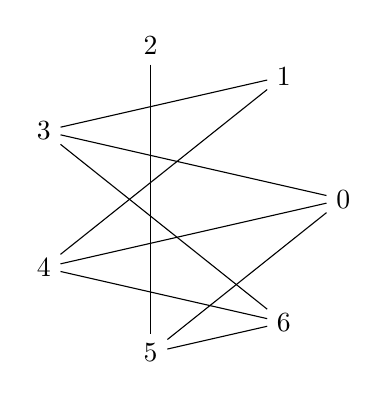
\begin{tikzpicture}
      \draw
        (0.0:2) node (0){0}
        (51.429:2) node (1){1}
        (102.857:2) node (2){2}
        (154.286:2) node (3){3}
        (205.714:2) node (4){4}
        (257.143:2) node (5){5}
        (308.571:2) node (6){6};
      \begin{scope}[-]
        \draw (0) to (3);
        \draw (0) to (4);
        \draw (0) to (5);
        \draw (1) to (3);
        \draw (1) to (4);
        \draw (2) to (5);
        \draw (3) to (6);
        \draw (4) to (6);
        \draw (5) to (6);
      \end{scope}
    \end{tikzpicture}
\end{figure}
\begin{itemize}
\item signature: 001110011000010001011
\item g: Graph with 7 nodes and 9 edges
\item order: 7
\item size: 9
\item max degree: 3
\item degrees: 1,2,3,3,3,3,3
\item is tree: 0
\item is bipartite: 1
\item has bridge: 1
\item is chordal: 0
\item is complete: 0
\item min cycle basis weight: 12
\item min cycle basis size: 3
\item diameter: 4
\item radius: 2
\item is eulerian: 0
\item is planar: 1
\item number of faces: 4
\item is regular: 0
\item p3: 16
\item p4: 8
\item property hash: 776b7e391d15246d51ac0ad59acd31878d0ae0c21619dc0e98db1ebee95fff22
\end{itemize}
\newpage
\begin{figure}
  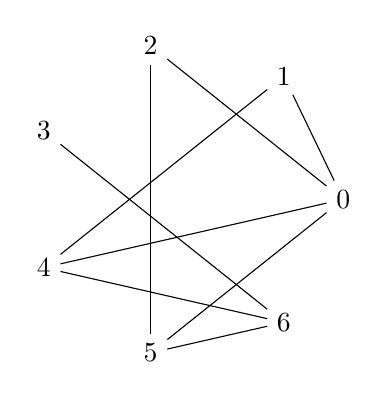
\begin{tikzpicture}
      \draw
        (0.0:2) node (0){0}
        (51.429:2) node (1){1}
        (102.857:2) node (2){2}
        (154.286:2) node (3){3}
        (205.714:2) node (4){4}
        (257.143:2) node (5){5}
        (308.571:2) node (6){6};
      \begin{scope}[-]
        \draw (0) to (1);
        \draw (0) to (2);
        \draw (0) to (4);
        \draw (0) to (5);
        \draw (1) to (4);
        \draw (2) to (5);
        \draw (3) to (6);
        \draw (4) to (6);
        \draw (5) to (6);
      \end{scope}
    \end{tikzpicture}
\end{figure}
\begin{itemize}
\item signature: 110110001000010001011
\item g: Graph with 7 nodes and 9 edges
\item order: 7
\item size: 9
\item max degree: 4
\item degrees: 1,2,2,3,3,3,4
\item is tree: 0
\item is bipartite: 0
\item has bridge: 1
\item is chordal: 0
\item is complete: 0
\item min cycle basis weight: 10
\item min cycle basis size: 3
\item diameter: 3
\item radius: 2
\item is eulerian: 0
\item is planar: 1
\item number of faces: 4
\item is regular: 0
\item p3: 11
\item p4: 8
\item property hash: 33f3f4402b24dc0a11f117cadec610407b913ab9609ed5085f43c123c3d72ad5
\end{itemize}
\newpage
\begin{figure}
  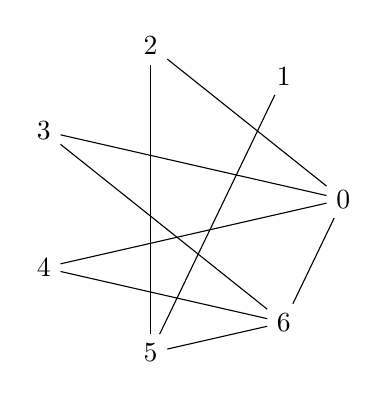
\begin{tikzpicture}
      \draw
        (0.0:2) node (0){0}
        (51.429:2) node (1){1}
        (102.857:2) node (2){2}
        (154.286:2) node (3){3}
        (205.714:2) node (4){4}
        (257.143:2) node (5){5}
        (308.571:2) node (6){6};
      \begin{scope}[-]
        \draw (0) to (2);
        \draw (0) to (3);
        \draw (0) to (4);
        \draw (0) to (6);
        \draw (1) to (5);
        \draw (2) to (5);
        \draw (3) to (6);
        \draw (4) to (6);
        \draw (5) to (6);
      \end{scope}
    \end{tikzpicture}
\end{figure}
\begin{itemize}
\item signature: 011101000100010001011
\item g: Graph with 7 nodes and 9 edges
\item order: 7
\item size: 9
\item max degree: 4
\item degrees: 1,2,2,2,3,4,4
\item is tree: 0
\item is bipartite: 0
\item has bridge: 1
\item is chordal: 0
\item is complete: 0
\item min cycle basis weight: 10
\item min cycle basis size: 3
\item diameter: 3
\item radius: 2
\item is eulerian: 0
\item is planar: 1
\item number of faces: 4
\item is regular: 0
\item p3: 12
\item p4: 8
\item property hash: ce268478adc4da93a09e9d3c88867da0f2b03662030d5c53a7b381f47907516e
\end{itemize}
\newpage
\begin{figure}
  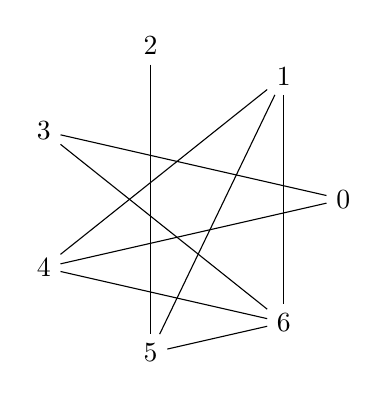
\begin{tikzpicture}
      \draw
        (0.0:2) node (0){0}
        (51.429:2) node (1){1}
        (102.857:2) node (2){2}
        (154.286:2) node (3){3}
        (205.714:2) node (4){4}
        (257.143:2) node (5){5}
        (308.571:2) node (6){6};
      \begin{scope}[-]
        \draw (0) to (3);
        \draw (0) to (4);
        \draw (1) to (4);
        \draw (1) to (5);
        \draw (1) to (6);
        \draw (2) to (5);
        \draw (3) to (6);
        \draw (4) to (6);
        \draw (5) to (6);
      \end{scope}
    \end{tikzpicture}
\end{figure}
\begin{itemize}
\item signature: 001100001110010001011
\item g: Graph with 7 nodes and 9 edges
\item order: 7
\item size: 9
\item max degree: 4
\item degrees: 1,2,2,3,3,3,4
\item is tree: 0
\item is bipartite: 0
\item has bridge: 1
\item is chordal: 0
\item is complete: 0
\item min cycle basis weight: 10
\item min cycle basis size: 3
\item diameter: 4
\item radius: 2
\item is eulerian: 0
\item is planar: 1
\item number of faces: 4
\item is regular: 0
\item p3: 11
\item p4: 8
\item property hash: 47a6f68401e3598f478a7f4047092ac4c602e3c44bc4a1e7a576121a63d1b89e
\end{itemize}
\newpage
\begin{figure}
  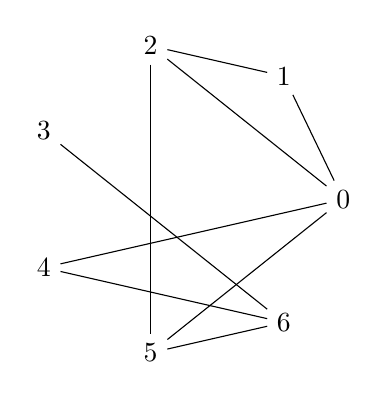
\begin{tikzpicture}
      \draw
        (0.0:2) node (0){0}
        (51.429:2) node (1){1}
        (102.857:2) node (2){2}
        (154.286:2) node (3){3}
        (205.714:2) node (4){4}
        (257.143:2) node (5){5}
        (308.571:2) node (6){6};
      \begin{scope}[-]
        \draw (0) to (1);
        \draw (0) to (2);
        \draw (0) to (4);
        \draw (0) to (5);
        \draw (1) to (2);
        \draw (2) to (5);
        \draw (3) to (6);
        \draw (4) to (6);
        \draw (5) to (6);
      \end{scope}
    \end{tikzpicture}
\end{figure}
\begin{itemize}
\item signature: 110110100000010001011
\item g: Graph with 7 nodes and 9 edges
\item order: 7
\item size: 9
\item max degree: 4
\item degrees: 1,2,2,3,3,3,4
\item is tree: 0
\item is bipartite: 0
\item has bridge: 1
\item is chordal: 0
\item is complete: 0
\item min cycle basis weight: 10
\item min cycle basis size: 3
\item diameter: 4
\item radius: 2
\item is eulerian: 0
\item is planar: 1
\item number of faces: 4
\item is regular: 0
\item p3: 11
\item p4: 8
\item property hash: 47a6f68401e3598f478a7f4047092ac4c602e3c44bc4a1e7a576121a63d1b89e
\end{itemize}
\newpage
\begin{figure}
  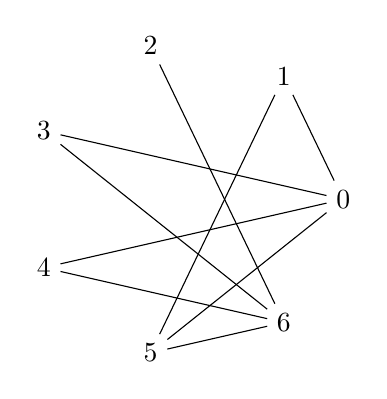
\begin{tikzpicture}
      \draw
        (0.0:2) node (0){0}
        (51.429:2) node (1){1}
        (102.857:2) node (2){2}
        (154.286:2) node (3){3}
        (205.714:2) node (4){4}
        (257.143:2) node (5){5}
        (308.571:2) node (6){6};
      \begin{scope}[-]
        \draw (0) to (1);
        \draw (0) to (3);
        \draw (0) to (4);
        \draw (0) to (5);
        \draw (1) to (5);
        \draw (2) to (6);
        \draw (3) to (6);
        \draw (4) to (6);
        \draw (5) to (6);
      \end{scope}
    \end{tikzpicture}
\end{figure}
\begin{itemize}
\item signature: 101110000100001001011
\item g: Graph with 7 nodes and 9 edges
\item order: 7
\item size: 9
\item max degree: 4
\item degrees: 1,2,2,2,3,4,4
\item is tree: 0
\item is bipartite: 0
\item has bridge: 1
\item is chordal: 0
\item is complete: 0
\item min cycle basis weight: 11
\item min cycle basis size: 3
\item diameter: 3
\item radius: 2
\item is eulerian: 0
\item is planar: 1
\item number of faces: 4
\item is regular: 0
\item p3: 15
\item p4: 8
\item property hash: c43608334aa7fbfdbddf2491b18e22af1fa58927d7402ff94c0df6431a7bf066
\end{itemize}
\newpage
\begin{figure}
  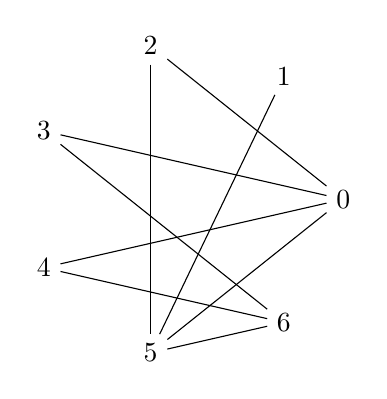
\begin{tikzpicture}
      \draw
        (0.0:2) node (0){0}
        (51.429:2) node (1){1}
        (102.857:2) node (2){2}
        (154.286:2) node (3){3}
        (205.714:2) node (4){4}
        (257.143:2) node (5){5}
        (308.571:2) node (6){6};
      \begin{scope}[-]
        \draw (0) to (2);
        \draw (0) to (3);
        \draw (0) to (4);
        \draw (0) to (5);
        \draw (1) to (5);
        \draw (2) to (5);
        \draw (3) to (6);
        \draw (4) to (6);
        \draw (5) to (6);
      \end{scope}
    \end{tikzpicture}
\end{figure}
\begin{itemize}
\item signature: 011110000100010001011
\item g: Graph with 7 nodes and 9 edges
\item order: 7
\item size: 9
\item max degree: 4
\item degrees: 1,2,2,2,3,4,4
\item is tree: 0
\item is bipartite: 0
\item has bridge: 1
\item is chordal: 0
\item is complete: 0
\item min cycle basis weight: 11
\item min cycle basis size: 3
\item diameter: 3
\item radius: 2
\item is eulerian: 0
\item is planar: 1
\item number of faces: 4
\item is regular: 0
\item p3: 15
\item p4: 8
\item property hash: c43608334aa7fbfdbddf2491b18e22af1fa58927d7402ff94c0df6431a7bf066
\end{itemize}
\newpage
\begin{figure}
  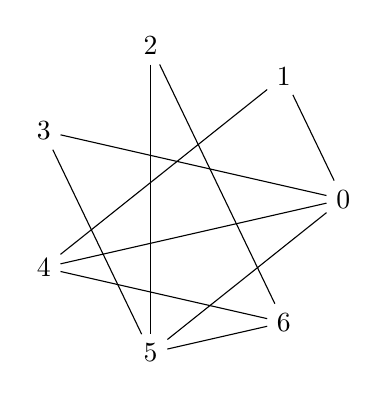
\begin{tikzpicture}
      \draw
        (0.0:2) node (0){0}
        (51.429:2) node (1){1}
        (102.857:2) node (2){2}
        (154.286:2) node (3){3}
        (205.714:2) node (4){4}
        (257.143:2) node (5){5}
        (308.571:2) node (6){6};
      \begin{scope}[-]
        \draw (0) to (1);
        \draw (0) to (3);
        \draw (0) to (4);
        \draw (0) to (5);
        \draw (1) to (4);
        \draw (2) to (5);
        \draw (2) to (6);
        \draw (3) to (5);
        \draw (4) to (6);
        \draw (5) to (6);
      \end{scope}
    \end{tikzpicture}
\end{figure}
\begin{itemize}
\item signature: 101110001000011010011
\item g: Graph with 7 nodes and 10 edges
\item order: 7
\item size: 10
\item max degree: 4
\item degrees: 2,2,2,3,3,4,4
\item is tree: 0
\item is bipartite: 0
\item has bridge: 0
\item is chordal: 0
\item is complete: 0
\item min cycle basis weight: 13
\item min cycle basis size: 4
\item diameter: 3
\item radius: 2
\item is eulerian: 0
\item is planar: 1
\item number of faces: 5
\item is regular: 0
\item p3: 12
\item p4: 8
\item property hash: 6cb7a6ec57c16c6cf83a98646022073d5de84b45dd82afc141d4a2096f8b23cd
\end{itemize}
\newpage
\begin{figure}
  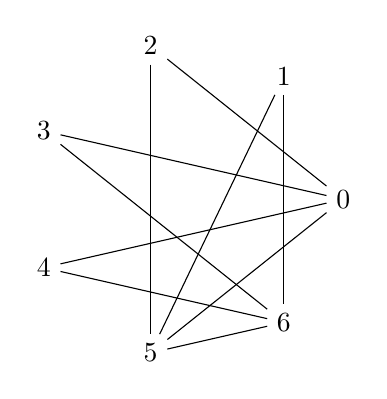
\begin{tikzpicture}
      \draw
        (0.0:2) node (0){0}
        (51.429:2) node (1){1}
        (102.857:2) node (2){2}
        (154.286:2) node (3){3}
        (205.714:2) node (4){4}
        (257.143:2) node (5){5}
        (308.571:2) node (6){6};
      \begin{scope}[-]
        \draw (0) to (2);
        \draw (0) to (3);
        \draw (0) to (4);
        \draw (0) to (5);
        \draw (1) to (5);
        \draw (1) to (6);
        \draw (2) to (5);
        \draw (3) to (6);
        \draw (4) to (6);
        \draw (5) to (6);
      \end{scope}
    \end{tikzpicture}
\end{figure}
\begin{itemize}
\item signature: 011110000110010001011
\item g: Graph with 7 nodes and 10 edges
\item order: 7
\item size: 10
\item max degree: 4
\item degrees: 2,2,2,2,4,4,4
\item is tree: 0
\item is bipartite: 0
\item has bridge: 0
\item is chordal: 0
\item is complete: 0
\item min cycle basis weight: 14
\item min cycle basis size: 4
\item diameter: 2
\item radius: 2
\item is eulerian: 1
\item is planar: 1
\item number of faces: 5
\item is regular: 0
\item p3: 16
\item p4: 8
\item property hash: 0aeb2b124349e924a5bbd209ef61404ec61914059225249749ca1d7f694ad088
\end{itemize}
\newpage
\begin{figure}
  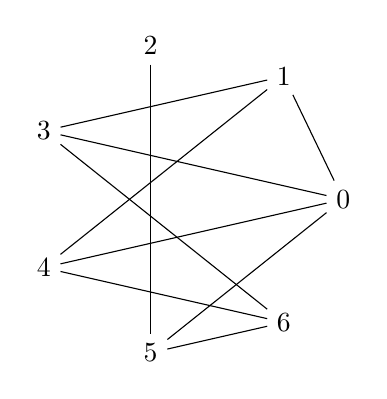
\begin{tikzpicture}
      \draw
        (0.0:2) node (0){0}
        (51.429:2) node (1){1}
        (102.857:2) node (2){2}
        (154.286:2) node (3){3}
        (205.714:2) node (4){4}
        (257.143:2) node (5){5}
        (308.571:2) node (6){6};
      \begin{scope}[-]
        \draw (0) to (1);
        \draw (0) to (3);
        \draw (0) to (4);
        \draw (0) to (5);
        \draw (1) to (3);
        \draw (1) to (4);
        \draw (2) to (5);
        \draw (3) to (6);
        \draw (4) to (6);
        \draw (5) to (6);
      \end{scope}
    \end{tikzpicture}
\end{figure}
\begin{itemize}
\item signature: 101110011000010001011
\item g: Graph with 7 nodes and 10 edges
\item order: 7
\item size: 10
\item max degree: 4
\item degrees: 1,3,3,3,3,3,4
\item is tree: 0
\item is bipartite: 0
\item has bridge: 1
\item is chordal: 0
\item is complete: 0
\item min cycle basis weight: 14
\item min cycle basis size: 4
\item diameter: 3
\item radius: 2
\item is eulerian: 0
\item is planar: 1
\item number of faces: 5
\item is regular: 0
\item p3: 15
\item p4: 8
\item property hash: d3b86db52629b9921b7618515f1ce529b237c3d4e8db8f2b990284080837e7cc
\end{itemize}
\newpage
\begin{figure}
  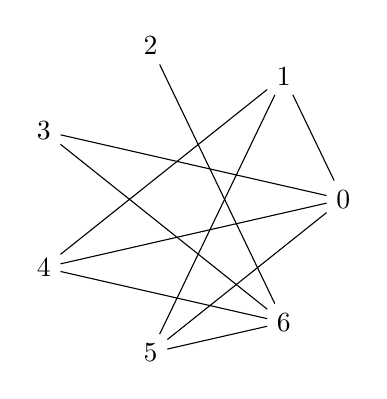
\begin{tikzpicture}
      \draw
        (0.0:2) node (0){0}
        (51.429:2) node (1){1}
        (102.857:2) node (2){2}
        (154.286:2) node (3){3}
        (205.714:2) node (4){4}
        (257.143:2) node (5){5}
        (308.571:2) node (6){6};
      \begin{scope}[-]
        \draw (0) to (1);
        \draw (0) to (3);
        \draw (0) to (4);
        \draw (0) to (5);
        \draw (1) to (4);
        \draw (1) to (5);
        \draw (2) to (6);
        \draw (3) to (6);
        \draw (4) to (6);
        \draw (5) to (6);
      \end{scope}
    \end{tikzpicture}
\end{figure}
\begin{itemize}
\item signature: 101110001100001001011
\item g: Graph with 7 nodes and 10 edges
\item order: 7
\item size: 10
\item max degree: 4
\item degrees: 1,2,3,3,3,4,4
\item is tree: 0
\item is bipartite: 0
\item has bridge: 1
\item is chordal: 0
\item is complete: 0
\item min cycle basis weight: 14
\item min cycle basis size: 4
\item diameter: 3
\item radius: 2
\item is eulerian: 0
\item is planar: 1
\item number of faces: 5
\item is regular: 0
\item p3: 16
\item p4: 8
\item property hash: 14f612159ea94a34bfa60bbd9d6b8d9c4be73821be5b63abe30cddf72bfc8c71
\end{itemize}
\newpage
\begin{figure}
  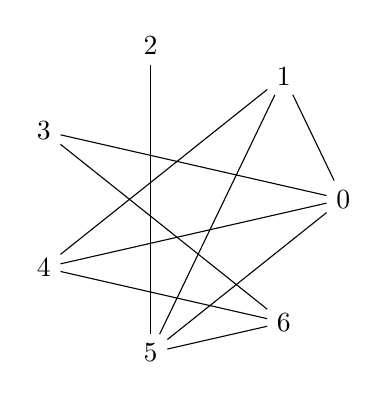
\begin{tikzpicture}
      \draw
        (0.0:2) node (0){0}
        (51.429:2) node (1){1}
        (102.857:2) node (2){2}
        (154.286:2) node (3){3}
        (205.714:2) node (4){4}
        (257.143:2) node (5){5}
        (308.571:2) node (6){6};
      \begin{scope}[-]
        \draw (0) to (1);
        \draw (0) to (3);
        \draw (0) to (4);
        \draw (0) to (5);
        \draw (1) to (4);
        \draw (1) to (5);
        \draw (2) to (5);
        \draw (3) to (6);
        \draw (4) to (6);
        \draw (5) to (6);
      \end{scope}
    \end{tikzpicture}
\end{figure}
\begin{itemize}
\item signature: 101110001100010001011
\item g: Graph with 7 nodes and 10 edges
\item order: 7
\item size: 10
\item max degree: 4
\item degrees: 1,2,3,3,3,4,4
\item is tree: 0
\item is bipartite: 0
\item has bridge: 1
\item is chordal: 0
\item is complete: 0
\item min cycle basis weight: 14
\item min cycle basis size: 4
\item diameter: 3
\item radius: 2
\item is eulerian: 0
\item is planar: 1
\item number of faces: 5
\item is regular: 0
\item p3: 16
\item p4: 8
\item property hash: 14f612159ea94a34bfa60bbd9d6b8d9c4be73821be5b63abe30cddf72bfc8c71
\end{itemize}
\newpage
\begin{figure}
  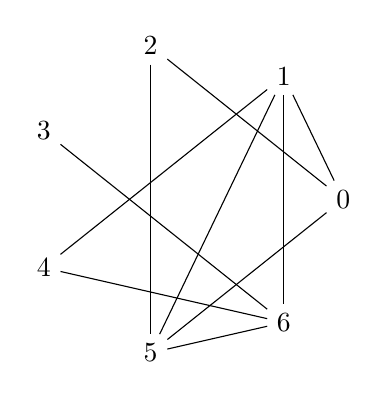
\begin{tikzpicture}
      \draw
        (0.0:2) node (0){0}
        (51.429:2) node (1){1}
        (102.857:2) node (2){2}
        (154.286:2) node (3){3}
        (205.714:2) node (4){4}
        (257.143:2) node (5){5}
        (308.571:2) node (6){6};
      \begin{scope}[-]
        \draw (0) to (1);
        \draw (0) to (2);
        \draw (0) to (5);
        \draw (1) to (4);
        \draw (1) to (5);
        \draw (1) to (6);
        \draw (2) to (5);
        \draw (3) to (6);
        \draw (4) to (6);
        \draw (5) to (6);
      \end{scope}
    \end{tikzpicture}
\end{figure}
\begin{itemize}
\item signature: 110010001110010001011
\item g: Graph with 7 nodes and 10 edges
\item order: 7
\item size: 10
\item max degree: 4
\item degrees: 1,2,2,3,4,4,4
\item is tree: 0
\item is bipartite: 0
\item has bridge: 1
\item is chordal: 1
\item is complete: 0
\item min cycle basis weight: 12
\item min cycle basis size: 4
\item diameter: 3
\item radius: 2
\item is eulerian: 0
\item is planar: 1
\item number of faces: 5
\item is regular: 0
\item p3: 11
\item p4: 8
\item property hash: 97c5462562e20db1d4aee8eca5ca29a8ba01e99bad2d9952dfc8f0e8bd4f3e28
\end{itemize}
\newpage
\begin{figure}
  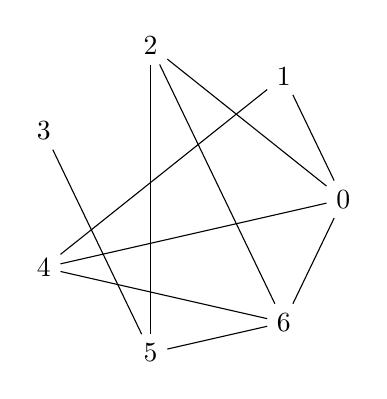
\begin{tikzpicture}
      \draw
        (0.0:2) node (0){0}
        (51.429:2) node (1){1}
        (102.857:2) node (2){2}
        (154.286:2) node (3){3}
        (205.714:2) node (4){4}
        (257.143:2) node (5){5}
        (308.571:2) node (6){6};
      \begin{scope}[-]
        \draw (0) to (1);
        \draw (0) to (2);
        \draw (0) to (4);
        \draw (0) to (6);
        \draw (1) to (4);
        \draw (2) to (5);
        \draw (2) to (6);
        \draw (3) to (5);
        \draw (4) to (6);
        \draw (5) to (6);
      \end{scope}
    \end{tikzpicture}
\end{figure}
\begin{itemize}
\item signature: 110101001000011010011
\item g: Graph with 7 nodes and 10 edges
\item order: 7
\item size: 10
\item max degree: 4
\item degrees: 1,2,3,3,3,4,4
\item is tree: 0
\item is bipartite: 0
\item has bridge: 1
\item is chordal: 1
\item is complete: 0
\item min cycle basis weight: 12
\item min cycle basis size: 4
\item diameter: 4
\item radius: 2
\item is eulerian: 0
\item is planar: 1
\item number of faces: 5
\item is regular: 0
\item p3: 10
\item p4: 8
\item property hash: bbe525a072df94e71c7de65183c959779e7a655aa64657b8030059fc8ac6be85
\end{itemize}
\newpage
\begin{figure}
  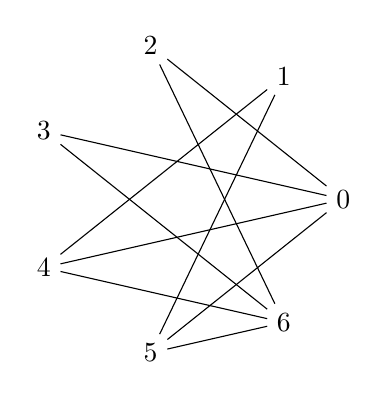
\begin{tikzpicture}
      \draw
        (0.0:2) node (0){0}
        (51.429:2) node (1){1}
        (102.857:2) node (2){2}
        (154.286:2) node (3){3}
        (205.714:2) node (4){4}
        (257.143:2) node (5){5}
        (308.571:2) node (6){6};
      \begin{scope}[-]
        \draw (0) to (2);
        \draw (0) to (3);
        \draw (0) to (4);
        \draw (0) to (5);
        \draw (1) to (4);
        \draw (1) to (5);
        \draw (2) to (6);
        \draw (3) to (6);
        \draw (4) to (6);
        \draw (5) to (6);
      \end{scope}
    \end{tikzpicture}
\end{figure}
\begin{itemize}
\item signature: 011110001100001001011
\item g: Graph with 7 nodes and 10 edges
\item order: 7
\item size: 10
\item max degree: 4
\item degrees: 2,2,2,3,3,4,4
\item is tree: 0
\item is bipartite: 1
\item has bridge: 0
\item is chordal: 0
\item is complete: 0
\item min cycle basis weight: 16
\item min cycle basis size: 4
\item diameter: 3
\item radius: 2
\item is eulerian: 0
\item is planar: 1
\item number of faces: 5
\item is regular: 0
\item p3: 21
\item p4: 8
\item property hash: e8cd7b9705c3f92759ed6ee602283acc77e28c38f100013366cae6e4b3ffd5e3
\end{itemize}
\newpage
\begin{figure}
  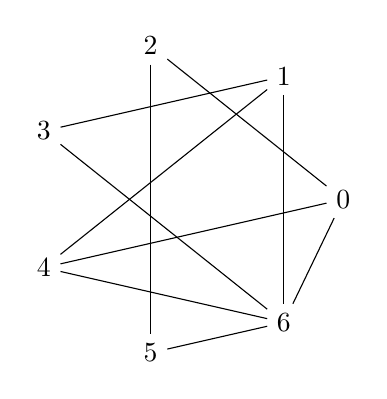
\begin{tikzpicture}
      \draw
        (0.0:2) node (0){0}
        (51.429:2) node (1){1}
        (102.857:2) node (2){2}
        (154.286:2) node (3){3}
        (205.714:2) node (4){4}
        (257.143:2) node (5){5}
        (308.571:2) node (6){6};
      \begin{scope}[-]
        \draw (0) to (2);
        \draw (0) to (4);
        \draw (0) to (6);
        \draw (1) to (3);
        \draw (1) to (4);
        \draw (1) to (6);
        \draw (2) to (5);
        \draw (3) to (6);
        \draw (4) to (6);
        \draw (5) to (6);
      \end{scope}
    \end{tikzpicture}
\end{figure}
\begin{itemize}
\item signature: 010101011010010001011
\item g: Graph with 7 nodes and 10 edges
\item order: 7
\item size: 10
\item max degree: 5
\item degrees: 2,2,2,3,3,3,5
\item is tree: 0
\item is bipartite: 0
\item has bridge: 0
\item is chordal: 0
\item is complete: 0
\item min cycle basis weight: 13
\item min cycle basis size: 4
\item diameter: 3
\item radius: 2
\item is eulerian: 0
\item is planar: 1
\item number of faces: 5
\item is regular: 0
\item p3: 13
\item p4: 8
\item property hash: a2e7cb536f5e85037e910f3d3c9d00a9f1d8f2ad92691a4339dc07d8fb9eed99
\end{itemize}
\newpage
\begin{figure}
  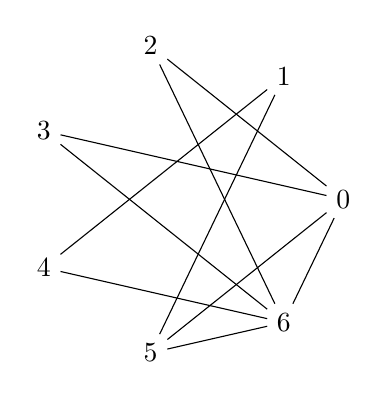
\begin{tikzpicture}
      \draw
        (0.0:2) node (0){0}
        (51.429:2) node (1){1}
        (102.857:2) node (2){2}
        (154.286:2) node (3){3}
        (205.714:2) node (4){4}
        (257.143:2) node (5){5}
        (308.571:2) node (6){6};
      \begin{scope}[-]
        \draw (0) to (2);
        \draw (0) to (3);
        \draw (0) to (5);
        \draw (0) to (6);
        \draw (1) to (4);
        \draw (1) to (5);
        \draw (2) to (6);
        \draw (3) to (6);
        \draw (4) to (6);
        \draw (5) to (6);
      \end{scope}
    \end{tikzpicture}
\end{figure}
\begin{itemize}
\item signature: 011011001100001001011
\item g: Graph with 7 nodes and 10 edges
\item order: 7
\item size: 10
\item max degree: 5
\item degrees: 2,2,2,2,3,4,5
\item is tree: 0
\item is bipartite: 0
\item has bridge: 0
\item is chordal: 0
\item is complete: 0
\item min cycle basis weight: 13
\item min cycle basis size: 4
\item diameter: 3
\item radius: 2
\item is eulerian: 0
\item is planar: 1
\item number of faces: 5
\item is regular: 0
\item p3: 14
\item p4: 8
\item property hash: c7de976b9cea8221c24f459b6f49f5db4e744bf536a7bf79b36442ec987c9846
\end{itemize}
\newpage
\begin{figure}
  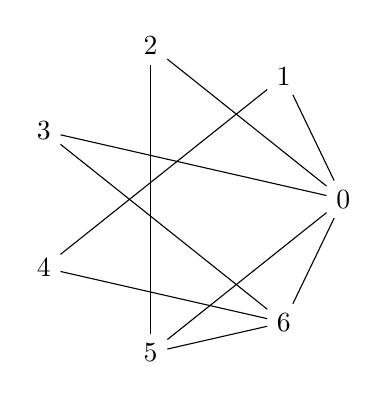
\begin{tikzpicture}
      \draw
        (0.0:2) node (0){0}
        (51.429:2) node (1){1}
        (102.857:2) node (2){2}
        (154.286:2) node (3){3}
        (205.714:2) node (4){4}
        (257.143:2) node (5){5}
        (308.571:2) node (6){6};
      \begin{scope}[-]
        \draw (0) to (1);
        \draw (0) to (2);
        \draw (0) to (3);
        \draw (0) to (5);
        \draw (0) to (6);
        \draw (1) to (4);
        \draw (2) to (5);
        \draw (3) to (6);
        \draw (4) to (6);
        \draw (5) to (6);
      \end{scope}
    \end{tikzpicture}
\end{figure}
\begin{itemize}
\item signature: 111011001000010001011
\item g: Graph with 7 nodes and 10 edges
\item order: 7
\item size: 10
\item max degree: 5
\item degrees: 2,2,2,2,3,4,5
\item is tree: 0
\item is bipartite: 0
\item has bridge: 0
\item is chordal: 0
\item is complete: 0
\item min cycle basis weight: 13
\item min cycle basis size: 4
\item diameter: 3
\item radius: 2
\item is eulerian: 0
\item is planar: 1
\item number of faces: 5
\item is regular: 0
\item p3: 14
\item p4: 8
\item property hash: c7de976b9cea8221c24f459b6f49f5db4e744bf536a7bf79b36442ec987c9846
\end{itemize}
\newpage
\begin{figure}
  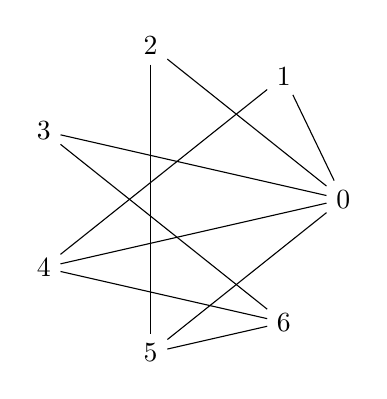
\begin{tikzpicture}
      \draw
        (0.0:2) node (0){0}
        (51.429:2) node (1){1}
        (102.857:2) node (2){2}
        (154.286:2) node (3){3}
        (205.714:2) node (4){4}
        (257.143:2) node (5){5}
        (308.571:2) node (6){6};
      \begin{scope}[-]
        \draw (0) to (1);
        \draw (0) to (2);
        \draw (0) to (3);
        \draw (0) to (4);
        \draw (0) to (5);
        \draw (1) to (4);
        \draw (2) to (5);
        \draw (3) to (6);
        \draw (4) to (6);
        \draw (5) to (6);
      \end{scope}
    \end{tikzpicture}
\end{figure}
\begin{itemize}
\item signature: 111110001000010001011
\item g: Graph with 7 nodes and 10 edges
\item order: 7
\item size: 10
\item max degree: 5
\item degrees: 2,2,2,3,3,3,5
\item is tree: 0
\item is bipartite: 0
\item has bridge: 0
\item is chordal: 0
\item is complete: 0
\item min cycle basis weight: 14
\item min cycle basis size: 4
\item diameter: 2
\item radius: 2
\item is eulerian: 0
\item is planar: 1
\item number of faces: 5
\item is regular: 0
\item p3: 16
\item p4: 8
\item property hash: 89c9cb6f0ce0f8ea39f703707477cc70c5d053c3893a92a27d5ede0e0e14feb2
\end{itemize}
\newpage
\begin{figure}
  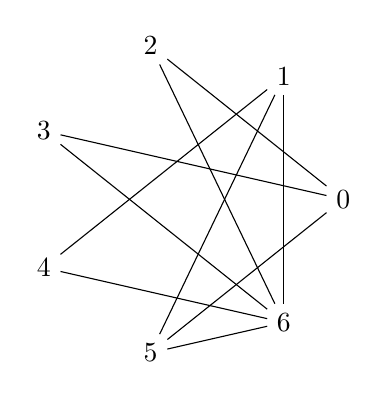
\begin{tikzpicture}
      \draw
        (0.0:2) node (0){0}
        (51.429:2) node (1){1}
        (102.857:2) node (2){2}
        (154.286:2) node (3){3}
        (205.714:2) node (4){4}
        (257.143:2) node (5){5}
        (308.571:2) node (6){6};
      \begin{scope}[-]
        \draw (0) to (2);
        \draw (0) to (3);
        \draw (0) to (5);
        \draw (1) to (4);
        \draw (1) to (5);
        \draw (1) to (6);
        \draw (2) to (6);
        \draw (3) to (6);
        \draw (4) to (6);
        \draw (5) to (6);
      \end{scope}
    \end{tikzpicture}
\end{figure}
\begin{itemize}
\item signature: 011010001110001001011
\item g: Graph with 7 nodes and 10 edges
\item order: 7
\item size: 10
\item max degree: 5
\item degrees: 2,2,2,3,3,3,5
\item is tree: 0
\item is bipartite: 0
\item has bridge: 0
\item is chordal: 0
\item is complete: 0
\item min cycle basis weight: 14
\item min cycle basis size: 4
\item diameter: 3
\item radius: 2
\item is eulerian: 0
\item is planar: 1
\item number of faces: 5
\item is regular: 0
\item p3: 16
\item p4: 8
\item property hash: 4304cf1c0c33875c1a4ae11cf2057e7b469ed0a61104ba0842c72c2285dacdeb
\end{itemize}
\newpage
\begin{figure}
  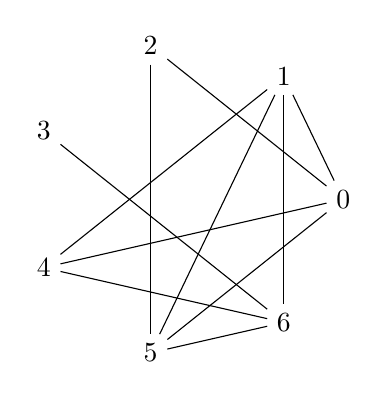
\begin{tikzpicture}
      \draw
        (0.0:2) node (0){0}
        (51.429:2) node (1){1}
        (102.857:2) node (2){2}
        (154.286:2) node (3){3}
        (205.714:2) node (4){4}
        (257.143:2) node (5){5}
        (308.571:2) node (6){6};
      \begin{scope}[-]
        \draw (0) to (1);
        \draw (0) to (2);
        \draw (0) to (4);
        \draw (0) to (5);
        \draw (1) to (4);
        \draw (1) to (5);
        \draw (1) to (6);
        \draw (2) to (5);
        \draw (3) to (6);
        \draw (4) to (6);
        \draw (5) to (6);
      \end{scope}
    \end{tikzpicture}
\end{figure}
\begin{itemize}
\item signature: 110110001110010001011
\item g: Graph with 7 nodes and 11 edges
\item order: 7
\item size: 11
\item max degree: 4
\item degrees: 1,2,3,4,4,4,4
\item is tree: 0
\item is bipartite: 0
\item has bridge: 1
\item is chordal: 0
\item is complete: 0
\item min cycle basis weight: 15
\item min cycle basis size: 5
\item diameter: 3
\item radius: 2
\item is eulerian: 0
\item is planar: 1
\item number of faces: 6
\item is regular: 0
\item p3: 13
\item p4: 8
\item property hash: 65b7eb49d96041e0c12f1ffee6577ea4087d32c6510ce7981f9d2ba6ca73f77a
\end{itemize}
\newpage
\begin{figure}
  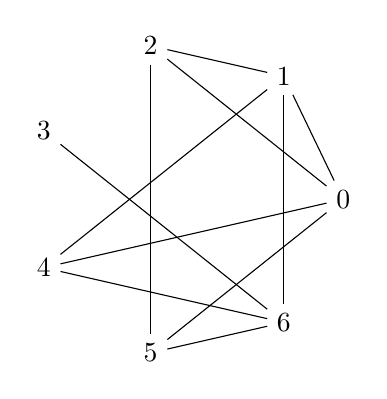
\begin{tikzpicture}
      \draw
        (0.0:2) node (0){0}
        (51.429:2) node (1){1}
        (102.857:2) node (2){2}
        (154.286:2) node (3){3}
        (205.714:2) node (4){4}
        (257.143:2) node (5){5}
        (308.571:2) node (6){6};
      \begin{scope}[-]
        \draw (0) to (1);
        \draw (0) to (2);
        \draw (0) to (4);
        \draw (0) to (5);
        \draw (1) to (2);
        \draw (1) to (4);
        \draw (1) to (6);
        \draw (2) to (5);
        \draw (3) to (6);
        \draw (4) to (6);
        \draw (5) to (6);
      \end{scope}
    \end{tikzpicture}
\end{figure}
\begin{itemize}
\item signature: 110110101010010001011
\item g: Graph with 7 nodes and 11 edges
\item order: 7
\item size: 11
\item max degree: 4
\item degrees: 1,3,3,3,4,4,4
\item is tree: 0
\item is bipartite: 0
\item has bridge: 1
\item is chordal: 0
\item is complete: 0
\item min cycle basis weight: 16
\item min cycle basis size: 5
\item diameter: 3
\item radius: 2
\item is eulerian: 0
\item is planar: 1
\item number of faces: 6
\item is regular: 0
\item p3: 15
\item p4: 8
\item property hash: 92c79d2927d979775591fe7a2d1688e1eb3d70456b58457475db665ec78961f8
\end{itemize}
\newpage
\begin{figure}
  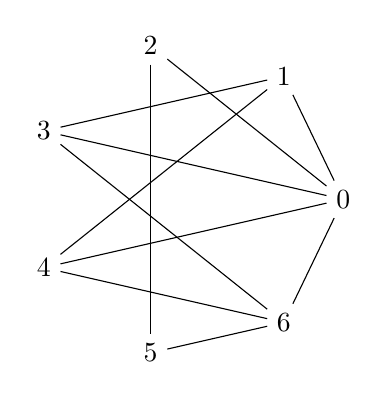
\begin{tikzpicture}
      \draw
        (0.0:2) node (0){0}
        (51.429:2) node (1){1}
        (102.857:2) node (2){2}
        (154.286:2) node (3){3}
        (205.714:2) node (4){4}
        (257.143:2) node (5){5}
        (308.571:2) node (6){6};
      \begin{scope}[-]
        \draw (0) to (1);
        \draw (0) to (2);
        \draw (0) to (3);
        \draw (0) to (4);
        \draw (0) to (6);
        \draw (1) to (3);
        \draw (1) to (4);
        \draw (2) to (5);
        \draw (3) to (6);
        \draw (4) to (6);
        \draw (5) to (6);
      \end{scope}
    \end{tikzpicture}
\end{figure}
\begin{itemize}
\item signature: 111101011000010001011
\item g: Graph with 7 nodes and 11 edges
\item order: 7
\item size: 11
\item max degree: 5
\item degrees: 2,2,3,3,3,4,5
\item is tree: 0
\item is bipartite: 0
\item has bridge: 0
\item is chordal: 0
\item is complete: 0
\item min cycle basis weight: 16
\item min cycle basis size: 5
\item diameter: 3
\item radius: 2
\item is eulerian: 0
\item is planar: 1
\item number of faces: 6
\item is regular: 0
\item p3: 15
\item p4: 8
\item property hash: cec7f6336f4ae1747f34e06af58d29f0b30913b54132bd977439976c66c1055f
\end{itemize}
\newpage
\begin{figure}
  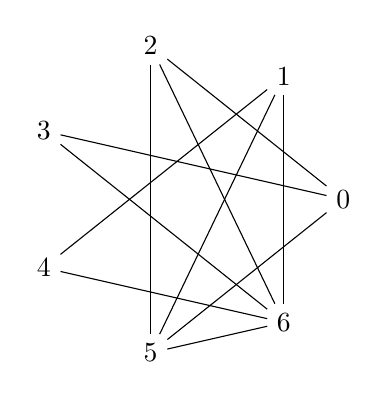
\begin{tikzpicture}
      \draw
        (0.0:2) node (0){0}
        (51.429:2) node (1){1}
        (102.857:2) node (2){2}
        (154.286:2) node (3){3}
        (205.714:2) node (4){4}
        (257.143:2) node (5){5}
        (308.571:2) node (6){6};
      \begin{scope}[-]
        \draw (0) to (2);
        \draw (0) to (3);
        \draw (0) to (5);
        \draw (1) to (4);
        \draw (1) to (5);
        \draw (1) to (6);
        \draw (2) to (5);
        \draw (2) to (6);
        \draw (3) to (6);
        \draw (4) to (6);
        \draw (5) to (6);
      \end{scope}
    \end{tikzpicture}
\end{figure}
\begin{itemize}
\item signature: 011010001110011001011
\item g: Graph with 7 nodes and 11 edges
\item order: 7
\item size: 11
\item max degree: 5
\item degrees: 2,2,3,3,3,4,5
\item is tree: 0
\item is bipartite: 0
\item has bridge: 0
\item is chordal: 0
\item is complete: 0
\item min cycle basis weight: 16
\item min cycle basis size: 5
\item diameter: 3
\item radius: 2
\item is eulerian: 0
\item is planar: 1
\item number of faces: 6
\item is regular: 0
\item p3: 15
\item p4: 8
\item property hash: cec7f6336f4ae1747f34e06af58d29f0b30913b54132bd977439976c66c1055f
\end{itemize}
\newpage
\begin{figure}
  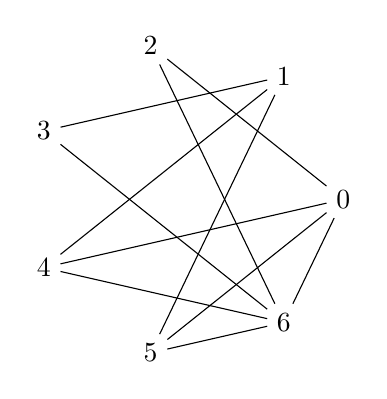
\begin{tikzpicture}
      \draw
        (0.0:2) node (0){0}
        (51.429:2) node (1){1}
        (102.857:2) node (2){2}
        (154.286:2) node (3){3}
        (205.714:2) node (4){4}
        (257.143:2) node (5){5}
        (308.571:2) node (6){6};
      \begin{scope}[-]
        \draw (0) to (2);
        \draw (0) to (4);
        \draw (0) to (5);
        \draw (0) to (6);
        \draw (1) to (3);
        \draw (1) to (4);
        \draw (1) to (5);
        \draw (2) to (6);
        \draw (3) to (6);
        \draw (4) to (6);
        \draw (5) to (6);
      \end{scope}
    \end{tikzpicture}
\end{figure}
\begin{itemize}
\item signature: 010111011100001001011
\item g: Graph with 7 nodes and 11 edges
\item order: 7
\item size: 11
\item max degree: 5
\item degrees: 2,2,3,3,3,4,5
\item is tree: 0
\item is bipartite: 0
\item has bridge: 0
\item is chordal: 0
\item is complete: 0
\item min cycle basis weight: 17
\item min cycle basis size: 5
\item diameter: 3
\item radius: 2
\item is eulerian: 0
\item is planar: 1
\item number of faces: 6
\item is regular: 0
\item p3: 18
\item p4: 8
\item property hash: 006d4b36cf2260194093a04d78d738b3d42c7884983f46e329f60ce986885f14
\end{itemize}
\newpage
\begin{figure}
  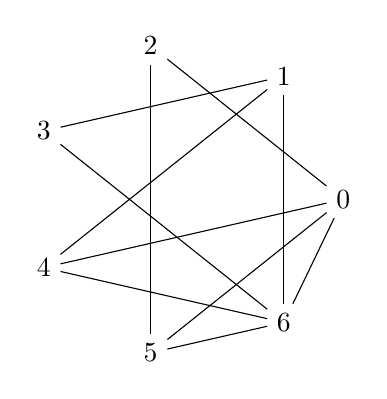
\begin{tikzpicture}
      \draw
        (0.0:2) node (0){0}
        (51.429:2) node (1){1}
        (102.857:2) node (2){2}
        (154.286:2) node (3){3}
        (205.714:2) node (4){4}
        (257.143:2) node (5){5}
        (308.571:2) node (6){6};
      \begin{scope}[-]
        \draw (0) to (2);
        \draw (0) to (4);
        \draw (0) to (5);
        \draw (0) to (6);
        \draw (1) to (3);
        \draw (1) to (4);
        \draw (1) to (6);
        \draw (2) to (5);
        \draw (3) to (6);
        \draw (4) to (6);
        \draw (5) to (6);
      \end{scope}
    \end{tikzpicture}
\end{figure}
\begin{itemize}
\item signature: 010111011010010001011
\item g: Graph with 7 nodes and 11 edges
\item order: 7
\item size: 11
\item max degree: 5
\item degrees: 2,2,3,3,3,4,5
\item is tree: 0
\item is bipartite: 0
\item has bridge: 0
\item is chordal: 1
\item is complete: 0
\item min cycle basis weight: 15
\item min cycle basis size: 5
\item diameter: 3
\item radius: 2
\item is eulerian: 0
\item is planar: 1
\item number of faces: 6
\item is regular: 0
\item p3: 12
\item p4: 8
\item property hash: f67a483b3363b1e55cc410be0881c2d1c85b1b9acb429d4cb370863497152d23
\end{itemize}
\newpage
\begin{figure}
  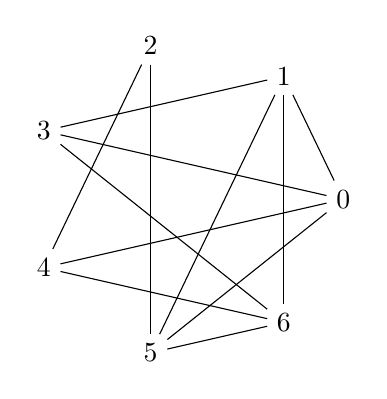
\begin{tikzpicture}
      \draw
        (0.0:2) node (0){0}
        (51.429:2) node (1){1}
        (102.857:2) node (2){2}
        (154.286:2) node (3){3}
        (205.714:2) node (4){4}
        (257.143:2) node (5){5}
        (308.571:2) node (6){6};
      \begin{scope}[-]
        \draw (0) to (1);
        \draw (0) to (3);
        \draw (0) to (4);
        \draw (0) to (5);
        \draw (1) to (3);
        \draw (1) to (5);
        \draw (1) to (6);
        \draw (2) to (4);
        \draw (2) to (5);
        \draw (3) to (6);
        \draw (4) to (6);
        \draw (5) to (6);
      \end{scope}
    \end{tikzpicture}
\end{figure}
\begin{itemize}
\item signature: 101110010110110001011
\item g: Graph with 7 nodes and 12 edges
\item order: 7
\item size: 12
\item max degree: 4
\item degrees: 2,3,3,4,4,4,4
\item is tree: 0
\item is bipartite: 0
\item has bridge: 0
\item is chordal: 0
\item is complete: 0
\item min cycle basis weight: 20
\item min cycle basis size: 6
\item diameter: 3
\item radius: 2
\item is eulerian: 0
\item is planar: 1
\item number of faces: 7
\item is regular: 0
\item p3: 19
\item p4: 8
\item property hash: a3ef46d91fb3246d078e8d0e104314889849d9c8ddf27c9ee47c6359ceecbba0
\end{itemize}
\newpage
\begin{figure}
  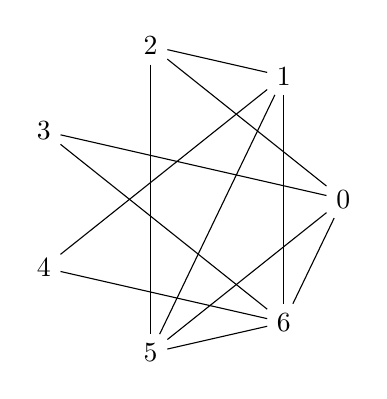
\begin{tikzpicture}
      \draw
        (0.0:2) node (0){0}
        (51.429:2) node (1){1}
        (102.857:2) node (2){2}
        (154.286:2) node (3){3}
        (205.714:2) node (4){4}
        (257.143:2) node (5){5}
        (308.571:2) node (6){6};
      \begin{scope}[-]
        \draw (0) to (2);
        \draw (0) to (3);
        \draw (0) to (5);
        \draw (0) to (6);
        \draw (1) to (2);
        \draw (1) to (4);
        \draw (1) to (5);
        \draw (1) to (6);
        \draw (2) to (5);
        \draw (3) to (6);
        \draw (4) to (6);
        \draw (5) to (6);
      \end{scope}
    \end{tikzpicture}
\end{figure}
\begin{itemize}
\item signature: 011011101110010001011
\item g: Graph with 7 nodes and 12 edges
\item order: 7
\item size: 12
\item max degree: 5
\item degrees: 2,2,3,4,4,4,5
\item is tree: 0
\item is bipartite: 0
\item has bridge: 0
\item is chordal: 0
\item is complete: 0
\item min cycle basis weight: 18
\item min cycle basis size: 6
\item diameter: 2
\item radius: 2
\item is eulerian: 0
\item is planar: 1
\item number of faces: 7
\item is regular: 0
\item p3: 15
\item p4: 8
\item property hash: cbd5b9cc78f9a3c444ddbda0bf1badf158f9d0420978de3fa5efc70072d2acec
\end{itemize}
\newpage
\begin{figure}
  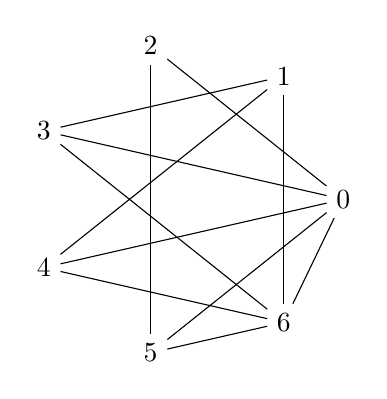
\begin{tikzpicture}
      \draw
        (0.0:2) node (0){0}
        (51.429:2) node (1){1}
        (102.857:2) node (2){2}
        (154.286:2) node (3){3}
        (205.714:2) node (4){4}
        (257.143:2) node (5){5}
        (308.571:2) node (6){6};
      \begin{scope}[-]
        \draw (0) to (2);
        \draw (0) to (3);
        \draw (0) to (4);
        \draw (0) to (5);
        \draw (0) to (6);
        \draw (1) to (3);
        \draw (1) to (4);
        \draw (1) to (6);
        \draw (2) to (5);
        \draw (3) to (6);
        \draw (4) to (6);
        \draw (5) to (6);
      \end{scope}
    \end{tikzpicture}
\end{figure}
\begin{itemize}
\item signature: 011111011010010001011
\item g: Graph with 7 nodes and 12 edges
\item order: 7
\item size: 12
\item max degree: 5
\item degrees: 2,3,3,3,3,5,5
\item is tree: 0
\item is bipartite: 0
\item has bridge: 0
\item is chordal: 0
\item is complete: 0
\item min cycle basis weight: 18
\item min cycle basis size: 6
\item diameter: 3
\item radius: 2
\item is eulerian: 0
\item is planar: 1
\item number of faces: 7
\item is regular: 0
\item p3: 15
\item p4: 8
\item property hash: 34d371582a6c1e89dedc0a415d85215a754badc9913a7541b868fe73afef65d5
\end{itemize}
\newpage
\begin{figure}
  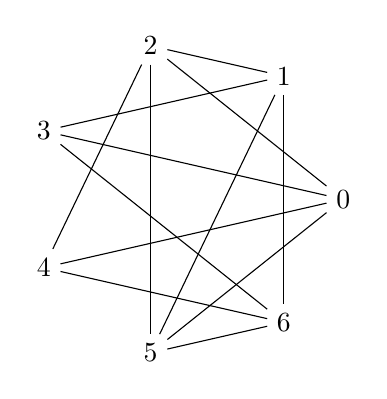
\begin{tikzpicture}
      \draw
        (0.0:2) node (0){0}
        (51.429:2) node (1){1}
        (102.857:2) node (2){2}
        (154.286:2) node (3){3}
        (205.714:2) node (4){4}
        (257.143:2) node (5){5}
        (308.571:2) node (6){6};
      \begin{scope}[-]
        \draw (0) to (2);
        \draw (0) to (3);
        \draw (0) to (4);
        \draw (0) to (5);
        \draw (1) to (2);
        \draw (1) to (3);
        \draw (1) to (5);
        \draw (1) to (6);
        \draw (2) to (4);
        \draw (2) to (5);
        \draw (3) to (6);
        \draw (4) to (6);
        \draw (5) to (6);
      \end{scope}
    \end{tikzpicture}
\end{figure}
\begin{itemize}
\item signature: 011110110110110001011
\item g: Graph with 7 nodes and 13 edges
\item order: 7
\item size: 13
\item max degree: 4
\item degrees: 3,3,4,4,4,4,4
\item is tree: 0
\item is bipartite: 0
\item has bridge: 0
\item is chordal: 0
\item is complete: 0
\item min cycle basis weight: 23
\item min cycle basis size: 7
\item diameter: 2
\item radius: 2
\item is eulerian: 0
\item is planar: 0
\item number of faces: 8
\item is regular: 0
\item p3: 21
\item p4: 8
\item property hash: a59584c94b29ce8e6ee6e579e9273bf28217f8edf40b0d93de65d69563ec3e98
\end{itemize}
\newpage
\begin{figure}
  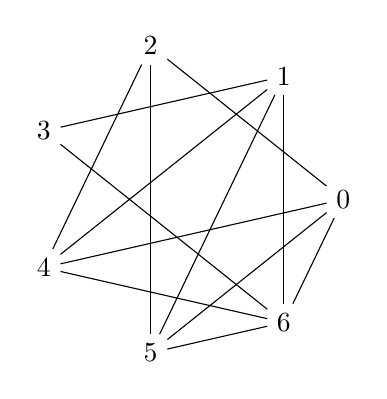
\begin{tikzpicture}
      \draw
        (0.0:2) node (0){0}
        (51.429:2) node (1){1}
        (102.857:2) node (2){2}
        (154.286:2) node (3){3}
        (205.714:2) node (4){4}
        (257.143:2) node (5){5}
        (308.571:2) node (6){6};
      \begin{scope}[-]
        \draw (0) to (2);
        \draw (0) to (4);
        \draw (0) to (5);
        \draw (0) to (6);
        \draw (1) to (3);
        \draw (1) to (4);
        \draw (1) to (5);
        \draw (1) to (6);
        \draw (2) to (4);
        \draw (2) to (5);
        \draw (3) to (6);
        \draw (4) to (6);
        \draw (5) to (6);
      \end{scope}
    \end{tikzpicture}
\end{figure}
\begin{itemize}
\item signature: 010111011110110001011
\item g: Graph with 7 nodes and 13 edges
\item order: 7
\item size: 13
\item max degree: 5
\item degrees: 2,3,4,4,4,4,5
\item is tree: 0
\item is bipartite: 0
\item has bridge: 0
\item is chordal: 0
\item is complete: 0
\item min cycle basis weight: 21
\item min cycle basis size: 7
\item diameter: 3
\item radius: 2
\item is eulerian: 0
\item is planar: 1
\item number of faces: 8
\item is regular: 0
\item p3: 17
\item p4: 8
\item property hash: 7294cbffecddaabb5e36c3f747ddb5dbe7f0a729fa7cac05d7dc30578074d6b5
\end{itemize}
\newpage
